% Dieser Text ist urheberrechtlich gesch�tzt
% Er stellt einen Auszug eines von mir erstellten Referates dar
% und darf nicht gewerblich genutzt werden
% die private bzw. Studiums bezogen Nutzung ist frei
% Januar 2006
% Autor: Sascha Frank 
% Universit�t Freiburg 
% www.informatik.uni-freiburg.de/~frank/
% www.namsu.de/


\documentclass[xcolor=dvipsnames]{beamer}
\usetheme{CambridgeUS}
%\usepackage{ngerman}
\usecolortheme{seagull}  
\usefonttheme{default}
%\usepackage[center]{caption}

\useoutertheme{infolines}
\useinnertheme{rectangles}

\usepackage{tikz}
%\usepackage{mathptmx}
\usepackage{cancel}
\usepackage{appendixnumberbeamer}



\title{The title}
\institute[]{~}
\date{\today}

\def\thisframelogos{}

\newcommand{\framelogo}[1]{\def\thisframelogos{#1}}

%\addtobeamertemplate{frametitle}{}{%
%	\begin{tikzpicture}[remember picture,overlay]
%	\node[anchor=north east,yshift=-8pt] at (current page.north east) {%
%		\foreach \img in \thisframelogos {%
%			\hspace{.5ex}%
%			\includegraphics[height=0.8cm]{\img}%
%		}%
%	};
%	\end{tikzpicture}}

%\setbeamercolor{alerted text}{fg=orange}
%\setbeamercolor{background canvas}{bg=white} %Hintergrund
%\setbeamercolor{block body alerted}{bg=normal text.bg!90!black} %BL�cke 
%%(block, exampleblock, alterblock)
%\setbeamercolor{block body}{bg=normal text.bg!90!black}
%\setbeamercolor{block body example}{bg=normal text.bg!90!black}
%\setbeamercolor{block title alerted}{use={normal text,alerted text},fg=alerted 
%text.fg!75!normal text.fg,bg=normal text.bg!75!black}
%\setbeamercolor{block title}{bg=blue} %Block hintergrund 1 
%\setbeamercolor{block title example}{use={normal text,example text},fg=example 
%text.fg!75!normal text.fg,bg=normal text.bg!75!black} %blok hintergrund 2
%\setbeamercolor{fine separation line}{}
%\setbeamercolor{frametitle}{fg=black} %frame titel
%\setbeamercolor{item projected}{fg=black}
%\setbeamercolor{normal text}{bg=black,fg=yellow}
%\setbeamercolor{palette sidebar primary}{use=normal text,fg=normal text.fg}
%\setbeamercolor{palette sidebar quaternary}{use=structure,fg=structure.fg}
%\setbeamercolor{palette sidebar secondary}{use=structure,fg=structure.fg}
%\setbeamercolor{palette sidebar tertiary}{use=normal text,fg=normal text.fg}
%\setbeamercolor{section in sidebar}{fg=brown}
%\setbeamercolor{section in sidebar shaded}{fg=grey}
%\setbeamercolor{separation line}{}
%\setbeamercolor{sidebar}{bg=blue}
%\setbeamercolor{sidebar}{parent=palette primary}
\definecolor{darkred}{rgb}{0.8,0,0}
\setbeamercolor{structure}{bg=white, fg=darkred}
%\setbeamercolor{subsection in sidebar}{fg=brown}
%\setbeamercolor{subsection in sidebar shaded}{fg=grey}
%\setbeamercolor{title}{fg=brown}
%\setbeamercolor{titlelike}{fg=brown}

\setbeamertemplate{itemize items}[default]


 %\renewcommand{\figurename}{}
\setbeamertemplate{caption}{\raggedright\insertcaption\par}
\defbeamertemplate*{sidebar right}{CambridgeUS}
{
	\vskip2pt%
	\llap{\insertlogo\hskip0.2cm}%
	\vfill
	\llap{\usebeamertemplate***{navigation symbols}\hskip0.2cm}%
	\vskip2pt%
}

\usepackage{lmodern}               
\usepackage{mathptmx}
%\usepackage{tpslifonts}
%\usepackage[perpage]{footmisc}
\begin{document}


\title[~]{Dynamical Decoupling of Nitrogen-Vacancy Electron Spins in Diamond and Nanodiamond} 
\author{Richard Kullmann} 
\date{26. Februar 2018}
%\logo{\includegraphics[scale=0.14]{husiegel}}
%\framelogo{husiegel}


\begin{frame}
\titlepage
\end{frame}



\section{Motivation}
\begin{frame}{Motivation}
\begin{columns}[t]
	\column{.5\textwidth}
	\centering
	\vspace{-0.5cm}
	\begin{figure}
		\includegraphics[scale=0.22]{intro31.pdf}
		\caption{magnetic imaging of a hard disk using NV centers, taken from \footnotemark[1]}
	\end{figure}
	\column{.5\textwidth}
	\centering
	\vspace{-1cm}
	\begin{figure}
		\includegraphics[scale=0.35]{intro41}
		\caption{wide-field image of magnetotactic bacteria, obtained with NV magnetometer, taken from \footnotemark[1]}
		
	\end{figure}
\end{columns}
\footnotetext[1]{L. Rondin et al., "Magnetometry with nitrogen-vacancy defects in diamond," \textit{Rep. Prog. Phys. 77}, 2014.}
\end{frame}

\begin{frame}{Motivation}
\begin{itemize}
	       \begin{columns}
		\column{0.58\linewidth}

		\item magnetometry: usage of single spins as quantum sensors
	\item sensitivity \footnotemark:
	\begin{equation}\nonumber
	\eta=\frac{\pi\hbar}{2 g\mu_B C\sqrt{N\cdot T_2}}
	\end{equation}
	$\rightarrow$ large $T_2$ time necessary for good resolution
	\item $T_2$ affected by interactions with surrounding spins 
	\item \textbf{Dynamical decoupling sequences}
	
		\column{0.38\linewidth}	\centering
			\begin{figure}	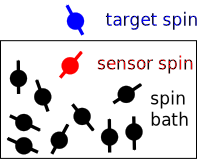
\includegraphics[height=3.5cm]{introneu.pdf}\caption{sensor spin in magnetic environment}
		\end{figure}

\end{columns} 
\end{itemize}
\footnotetext{{L. M. Pham, \textit{Magnetic Field Sensing with Nitrogen-Vacancy Color Centers in Diamond}. PhD thesis, The School of Engineering and Applied Sciences, 2013.}}
\end{frame}
%\begin{frame}{Contents}
%\tableofcontents
%\end{frame}
\section{Theory}
\subsection{NV center}
\begin{frame}{NV center}
\vspace{-1cm}
\begin{columns}[t]
\column{.5\textwidth}
\centering
\begin{figure}
\includegraphics[scale=0.3]{nv.pdf}
\caption{structure of an NV center, taken from \footnotemark[1]}
\end{figure}
\column{.5\textwidth}
\centering
\begin{figure}
\includegraphics[scale=0.2]{el}
\caption{NV energy level scheme, taken from \footnotemark[2]}

\end{figure}
\end{columns}
\begin{itemize}
\item $m_s=0$ and $m_s=\pm1$ sublevels separated by D=2.87GHz
\item fluorescence with ZPL at 637 nm
\item $m_s=0$: bright state, $m_s=\pm1$: dark state
\end{itemize}			      
    	\footnotetext[1]{{L. Rondin et al., "Magnetometry with nitrogen-vacancy defects in diamond," \textit{Rep. Prog. Phys. 77}, 2014.}}	\footnotetext[2]{{R. Hanson et al., "Room-temperature manipulation and decoherence of a single
    			spin in diamond,"\textit{ Physical Review B 74}, 2006.}}
\end{frame}

\subsection{Rabi oscillations}
%\begin{frame}{Rabi oscillations}
%\begin{itemize}
%	\item single electronis spin in static magnetic field:
%	\begin{equation}\label{hz}
%	\hat{H}_Z=-\gamma_S\hat{S}\hat{B}=-\gamma_S\hat{S}_zB_z=-\frac{\gamma_S\hbar B_z}{2}\hat{\sigma}_z=\frac{\hbar}{2}\omega_B\hat{\sigma}_z
%	\end{equation}
%	\item adding oscillating field:
%	\begin{equation}
%	\hat{B}=B_1(\hat{x}\cos\omega t-\hat{y}\sin\omega t)\Rightarrow \hat{H}_B=-\gamma B_1(\hat{S}_x\cos\omega t-\hat{S}_y\sin\omega t)
%	\end{equation}
%	\item total Hamiltonian:
%	\begin{equation}
%	\hat{H}=\hat{H}_Z+\hat{H}_B=\frac{\hbar}{2}\left(\begin{matrix}
%	\omega_{B}&-\omega_1e^{i\omega t}\\
%	-\omega_1e^{-i\omega t}&-\omega_ {B}
%	\end{matrix}\right)
%	\end{equation}
%\end{itemize}
%\end{frame}

\begin{frame}{Rabi oscillations}
	\begin{itemize}
	\begin{columns}
		\column{0.58\linewidth}	
		\item two level system with AC magnetic field
		\item Rabi's formula for resonant excitation:
	\begin{equation}\nonumber
	P_{1\rightarrow 0}(t)=\sin^2\left(\frac{\omega_1 t}{2}\right)
	\end{equation}
	\vspace{-0.5cm}
	\begin{figure}	\includegraphics[height=4cm]{rabis2.pdf}\caption{Rabi oscillations under resonant excitation}
	\end{figure}
	
		\column{0.38\linewidth}	\centering
		\begin{Huge}$\curvearrowright$\end{Huge}\textbf{ $\pi$ and $\pi/2$ pulses}
		\begin{figure}	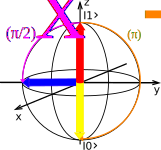
\includegraphics[height=4cm]{bloch.pdf}\caption{rotations on the Bloch sphere}
		\end{figure}	
	\end{columns} 
	\end{itemize}

\end{frame}

\subsection{Dynamical decoupling sequences}

\begin{frame}{Dynamical decoupling sequences}
		\begin{Large} Hahn Echo \end{Large}
		\begin{itemize}
	\item cancels slowly varying inhomogeneities
			\begin{figure}
				\includegraphics[scale=0.5]{Hahn2}
			\end{figure}
\end{itemize}
			\begin{Large} CPMG \end{Large}
\begin{itemize}
			\item single axis rotations
			\item higher decoupling efficiency than Hahn Echo
			\begin{figure}
			
\includegraphics[scale=0.4]{CPMG41}\caption{CPMG-4 pulse sequence}
		\end{figure}
			
\end{itemize}
\end{frame}

\begin{frame}{Dynamical decoupling sequences}
	\begin{Large} XY \end{Large}
\begin{itemize}
	\item CPMG pulse spacing
	\item alternating $\pi_x$ and $\pi_y$ pulses perform 3D decoupling
	\begin{figure}
		
		
\includegraphics[scale=0.4]{XY81}
		\vspace{-0.2cm}
		\caption{XY-8 sequence: red pulses are $\pi_y$ and blue pulses are $\pi_x$}
		\vspace{-0.3cm}
	\end{figure}
\end{itemize}
\begin{Large} UDD \end{Large}
\begin{itemize}

	\item no equidistant spacings
\begin{figure}
	\includegraphics[scale=0.4]{UDD1}\vspace{-0.3cm}\caption{UDD-6 sequence}
\end{figure}
\end{itemize}
\end{frame}


\section{Setup}
\begin{frame}{Setup} 
\begin{figure}
	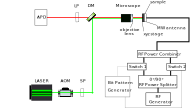
\includegraphics[scale=0.6]{setup5}
\end{figure}

\end{frame}
\section{Measurements}
\subsection{Nanodiamond}
\begin{frame}{Resonance scan and Hahn Echo}
\begin{center}
	\vspace{-1cm}
	\begin{tikzpicture}
	\node (img1)[xshift=-2.5cm][yshift=3cm] {\includegraphics[scale=0.4]{rf2fit.pdf}};\pause
	\node (img2) at (img1.north west)[yshift=-2.5cm][xshift=0.5cm] {\includegraphics[scale=0.3]{rabinano2.pdf}};\pause
	\node (img3) at (img1.south west)[yshift=0cm][xshift=0.5cm] {\includegraphics[scale=0.3]{Hahnn111.pdf}};
	\node[draw] at (img3.south east)[yshift=1cm][xshift=2cm] {$T_{2,H}$=(2.41$\pm$0.12)$\mu$s};
	\end{tikzpicture}
	
\end{center}

	

\end{frame}



\begin{frame}{CPMG}
\vspace{-5.5cm}
\begin{columns}[t]
	\column{1\textwidth}
	\centering
\begin{figure}
	\includegraphics[scale=0.5]{4cpmgo1pt.pdf}\caption{Comparison of CPMG-sequences with different numbers of pulses}
\end{figure}
\vspace{-5cm}

\begin{table}[H]
	\centering
	\scalebox{0.8}{	
	\begin{tabular}{l|l|l}
		sequence              & $T_2$ {[}ns{]}  & $T_2/T_{2,H}$                     \\\hline
		CPMG-8   &  12900           $\pm$ 1100 & 5.35\\
		CPMG-16  &  17500            $\pm$ 1400 &7.26\\
		CPMG-32  &  31700         $\pm$ 3700 & 13.14\\
		CPMG-64  & 38100        $\pm$ 1200 & 15.80
	\end{tabular}}
\end{table}
\vspace{-6cm}
	\begin{figure}
	
\includegraphics[scale=0.2]{CPMG42}
\end{figure}


\end{columns}
\end{frame}

\begin{frame}{XY}
\vspace{-2cm}
\begin{columns}[t]
	\column{1\textwidth}
	\centering
	\begin{figure}
		\includegraphics[scale=0.5]{nanox.pdf}\caption{Comparison of XY-sequences with different numbers of pulses}
	\end{figure}
	\vspace{-5cm}
	
	\begin{table}[H]
		\centering
		\scalebox{0.8}{	
			\begin{tabular}{l|l|l}
				sequence&		$T_{2}$ {[}ns{]}	&$T_{2}/T_{2,H}$\\\hline
				XY-8	 &	10400          $\pm$ 1400&	4.33\\
				XY-16&	13700          $\pm$1600	&5.68\\
				XY-32&		9900        $\pm$ 2400& 	4.09\\
				XY-64&14000         $\pm$ 2200&	5.79\\
		\end{tabular}}
	\end{table}
	\vspace{-6.5cm}
	\begin{figure}
		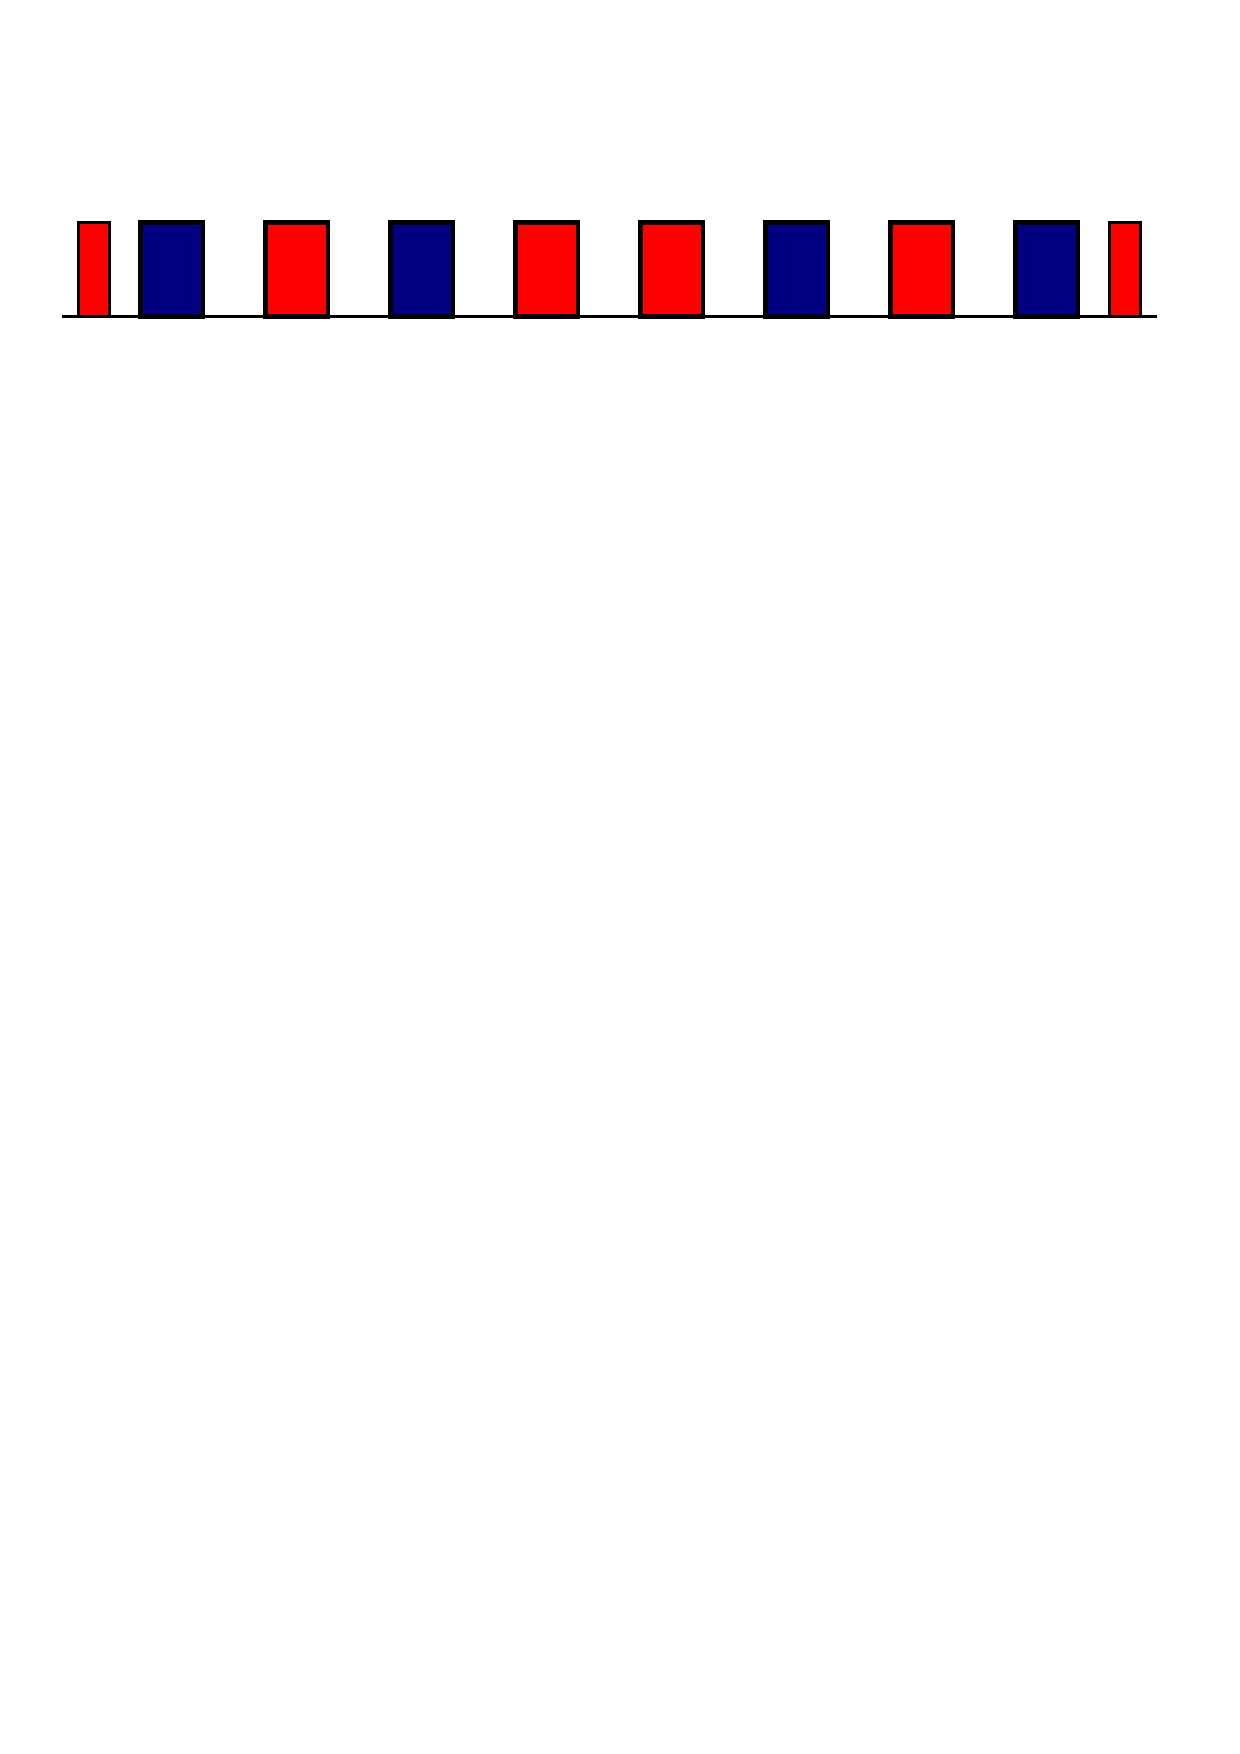
\includegraphics[scale=0.2]{XY82}
	\end{figure}
\end{columns}
\end{frame}
\begin{frame}{UDD}
\vspace{-2.5cm}
\begin{columns}[t]
	\column{1\textwidth}
	\begin{figure}
		\includegraphics[scale=0.5]{udd3.pdf}\caption{Performance of UDD on nanodiamond}
	\end{figure}


	\vspace{-9cm}

		\begin{figure}
			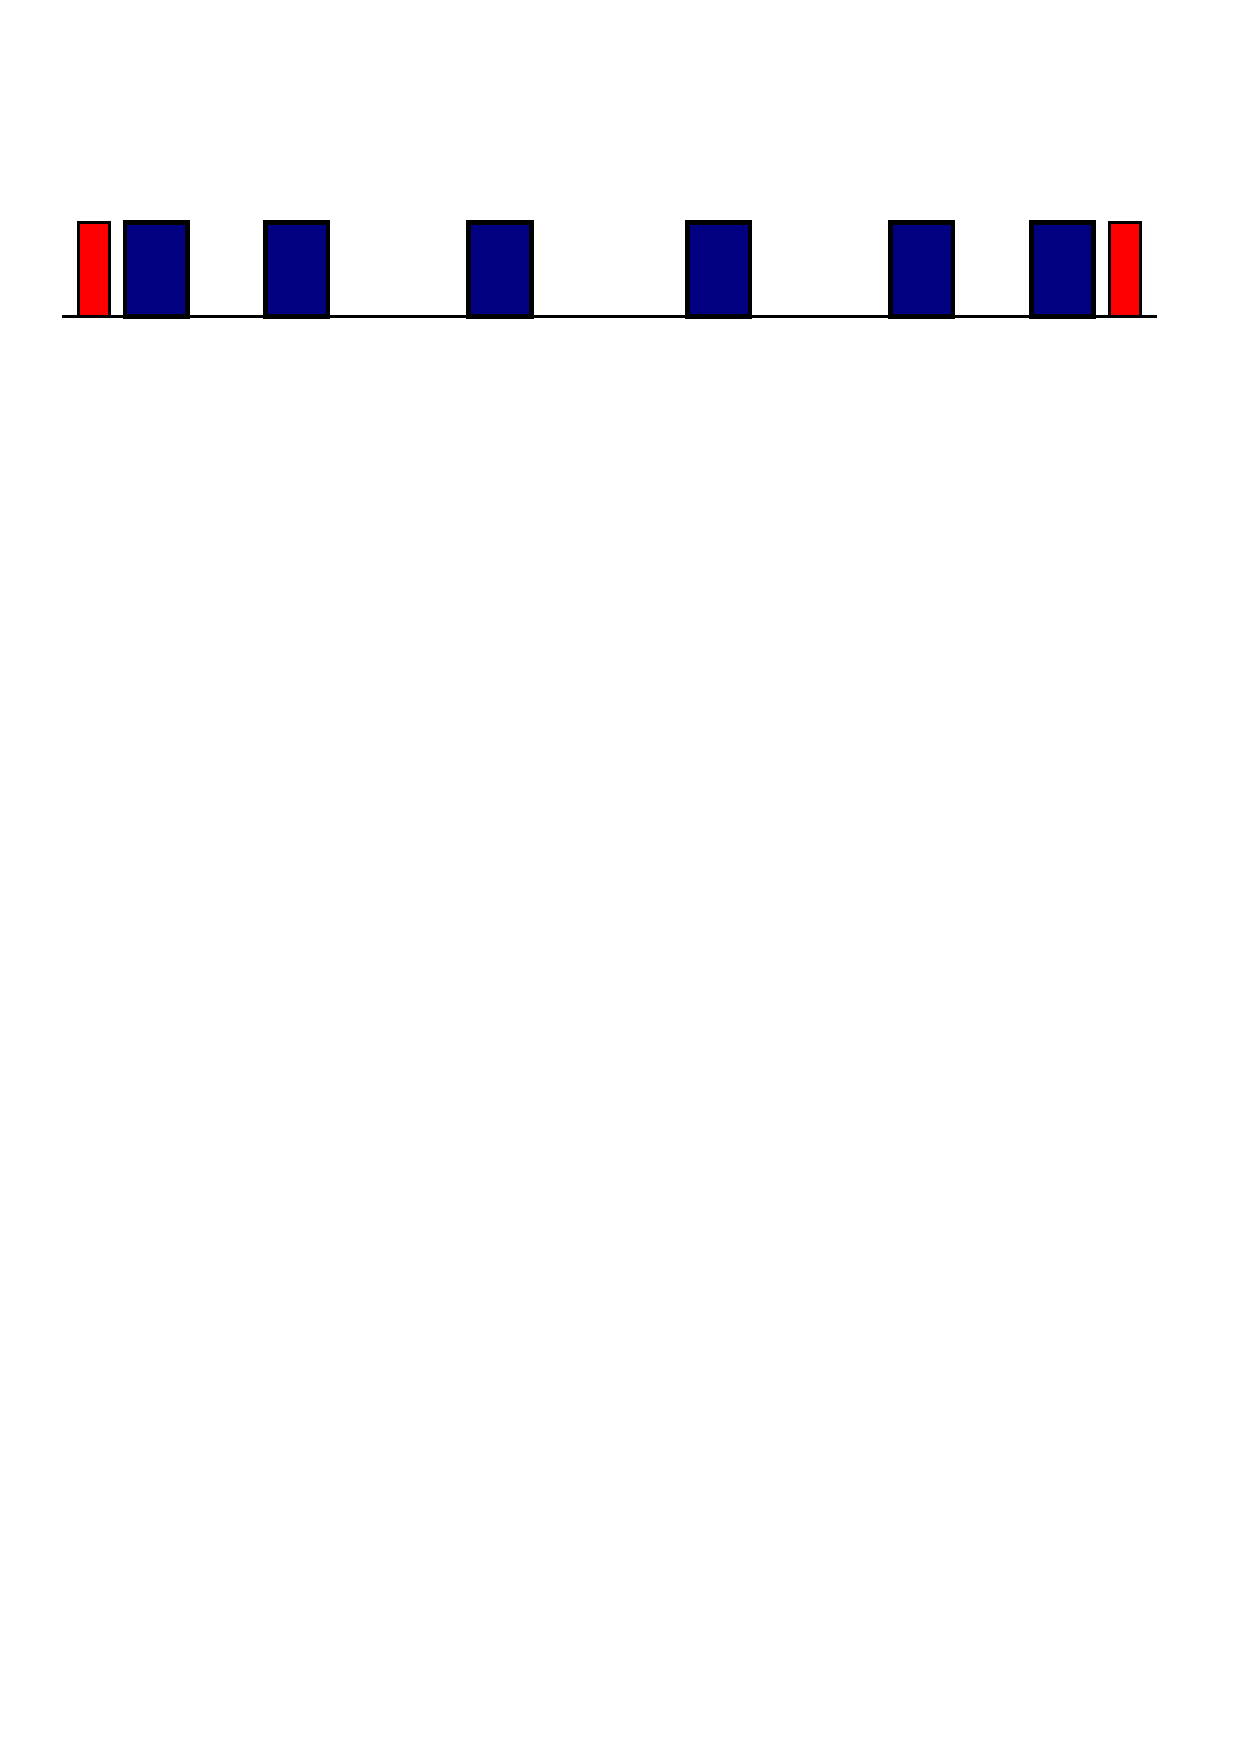
\includegraphics[scale=0.2]{UDD2}
		\end{figure}
	\vspace{-2cm}
		\begin{table}[H]
		\centering
		\scalebox{0.9}{	
			\begin{tabular}{l|l}
		$T_{2}$ {[}ns{]}	&$T_{2}/T_{2,H}$\\\hline
				10600          $\pm$ 900&	4.39\\
			\end{tabular}}
		\end{table}
\end{columns}
\end{frame}
\begin{frame}{Different NVs}

\begin{columns}[t]
	\column{.5\textwidth}
	\centering
	\includegraphics[scale=0.23]{cv2.pdf}\\
	\includegraphics[scale=0.23]{xv2.pdf}
	\column{.5\textwidth}
	\centering
	\vspace{-4cm}
	\begin{table}[H]
		\centering
		\caption{CPMG-8 for different NVs}
		\begin{tabular}{l|l|l}
				&  $T_{2}$ {[}ns{]}                                              & $T_{2}$/$T_{2,H}$             \\\hline
			NV 1             & 12900            $\pm$ 1100         & 5.35 \\
			NV 2             & 5000           $\pm$ 200       & 3.45 \\
			NV 3            & 14700         $\pm$ 1400         & 16.63
		\end{tabular}
	\end{table}

	\begin{table}[H]
		\centering
		\caption{XY-8 for different NVs}
		\begin{tabular}{l|l|l}
			&  $T_{2}$ {[}ns{]}                                              & $T_{2}$/$T_{2,H}$              \\\hline
			NV 1             & 10700         $\pm$ 1000         & 4.42 \\
			NV 2             & 4600         $\pm$ 200        & 3.18 \\
			NV 3            & 17000        $\pm$ 2000         & 19.42
		\end{tabular}
	\end{table}
\end{columns}
\end{frame}

\begin{frame}{Comparison of XY and CPMG}

\begin{figure}
	\includegraphics[scale=0.5]{xcvergleich.pdf}\caption{performance of XY and CPMG on nanodiamonds}
\end{figure}
\end{frame}


\subsection{Bulk diamond}
%\begin{frame}{Resonance scan and Hahn Echo}
%\begin{center}
%	\vspace{-1cm}
%	\begin{tikzpicture}
%	\node (img1)[xshift=-2.5cm][yshift=3cm] {\includegraphics[scale=0.4]{rfbulk.pdf}};\pause
%	\node (img2) at (img1.north east)[yshift=-2.5cm][xshift=-0.5cm] {\includegraphics[scale=0.3]{bulkrabi.pdf}};\pause
%	\node (img3) at (img1.south east)[yshift=0cm][xshift=-0.5cm] {\includegraphics[scale=0.3]{bulkhahn.pdf}};
%	\node[draw] at (img3.south west)[yshift=1.7cm][xshift=-2.5cm] {$T_2$(all points)=(235$\pm$13)ns};
%	\node[draw] at (img3.south west)[yshift=0.7cm][xshift=-2.5cm]{$T_2(t\leq 600\text{ns})$=(302$\pm$25)ns};
%	\end{tikzpicture}
%	
%\end{center}
%
%
%
%\end{frame}

%\begin{frame}{CPMG}
%\vspace{-2cm}
%\begin{columns}[t]
%	\column{1\textwidth}
%	\centering
%	\begin{figure}
%		\includegraphics[scale=0.5]{cpbulk.pdf}\caption{Comparison of CPMG-sequences with different numbers of pulses}
%	\end{figure}
%	\vspace{-8.3cm}
%	
%	\begin{table}[H]
%		\centering
%		\scalebox{0.8}{	
%			\begin{tabular}{l|ll}
%				pulses &    coherence time {[}ns{]}   & $t_0$/$T_2$   \\\hline
%				4                &    17200$\pm$ 700                      & 57 \\
%				8                &    23100$\pm$ 1100                    & 77\\
%				16               &    44500$\pm$ 1900                     & 148 \\
%				32               &    59500$\pm$ 3100                     & 197
%		\end{tabular}}
%	\end{table}
%	\vspace{2.2cm}
%	\begin{figure}
%		
\includegraphics[scale=0.2]{CPMG42}
%	\end{figure}
%	
%	
%\end{columns}
%\end{frame}

%\begin{frame}{XY}
%\vspace{-1cm}
%\begin{columns}[t]
%	\column{1\textwidth}
%	\centering
%	\begin{figure}
%		\includegraphics[scale=0.5]{xybulk.pdf}\caption{Comparison of XY-sequences with different numbers of pulses}
%	\end{figure}
%	\vspace{-8.3cm}
%	
%	\begin{table}[H]
%		\centering
%		\scalebox{0.8}{	
%			\begin{tabular}{l|lll}
%				number of pulses &    coherence time {[}ns{]}   & $t_0$/$T_2$   \\\hline
%				8                &    28500$\pm$ 1700                    & 94\\
%				16               &    29600$\pm$ 1200                     & 98 \\
%				32               &    24500$\pm$ 1400                     & 81
%		\end{tabular}}
%	\end{table}
%	\vspace{-1cm}
%	\begin{figure}
%		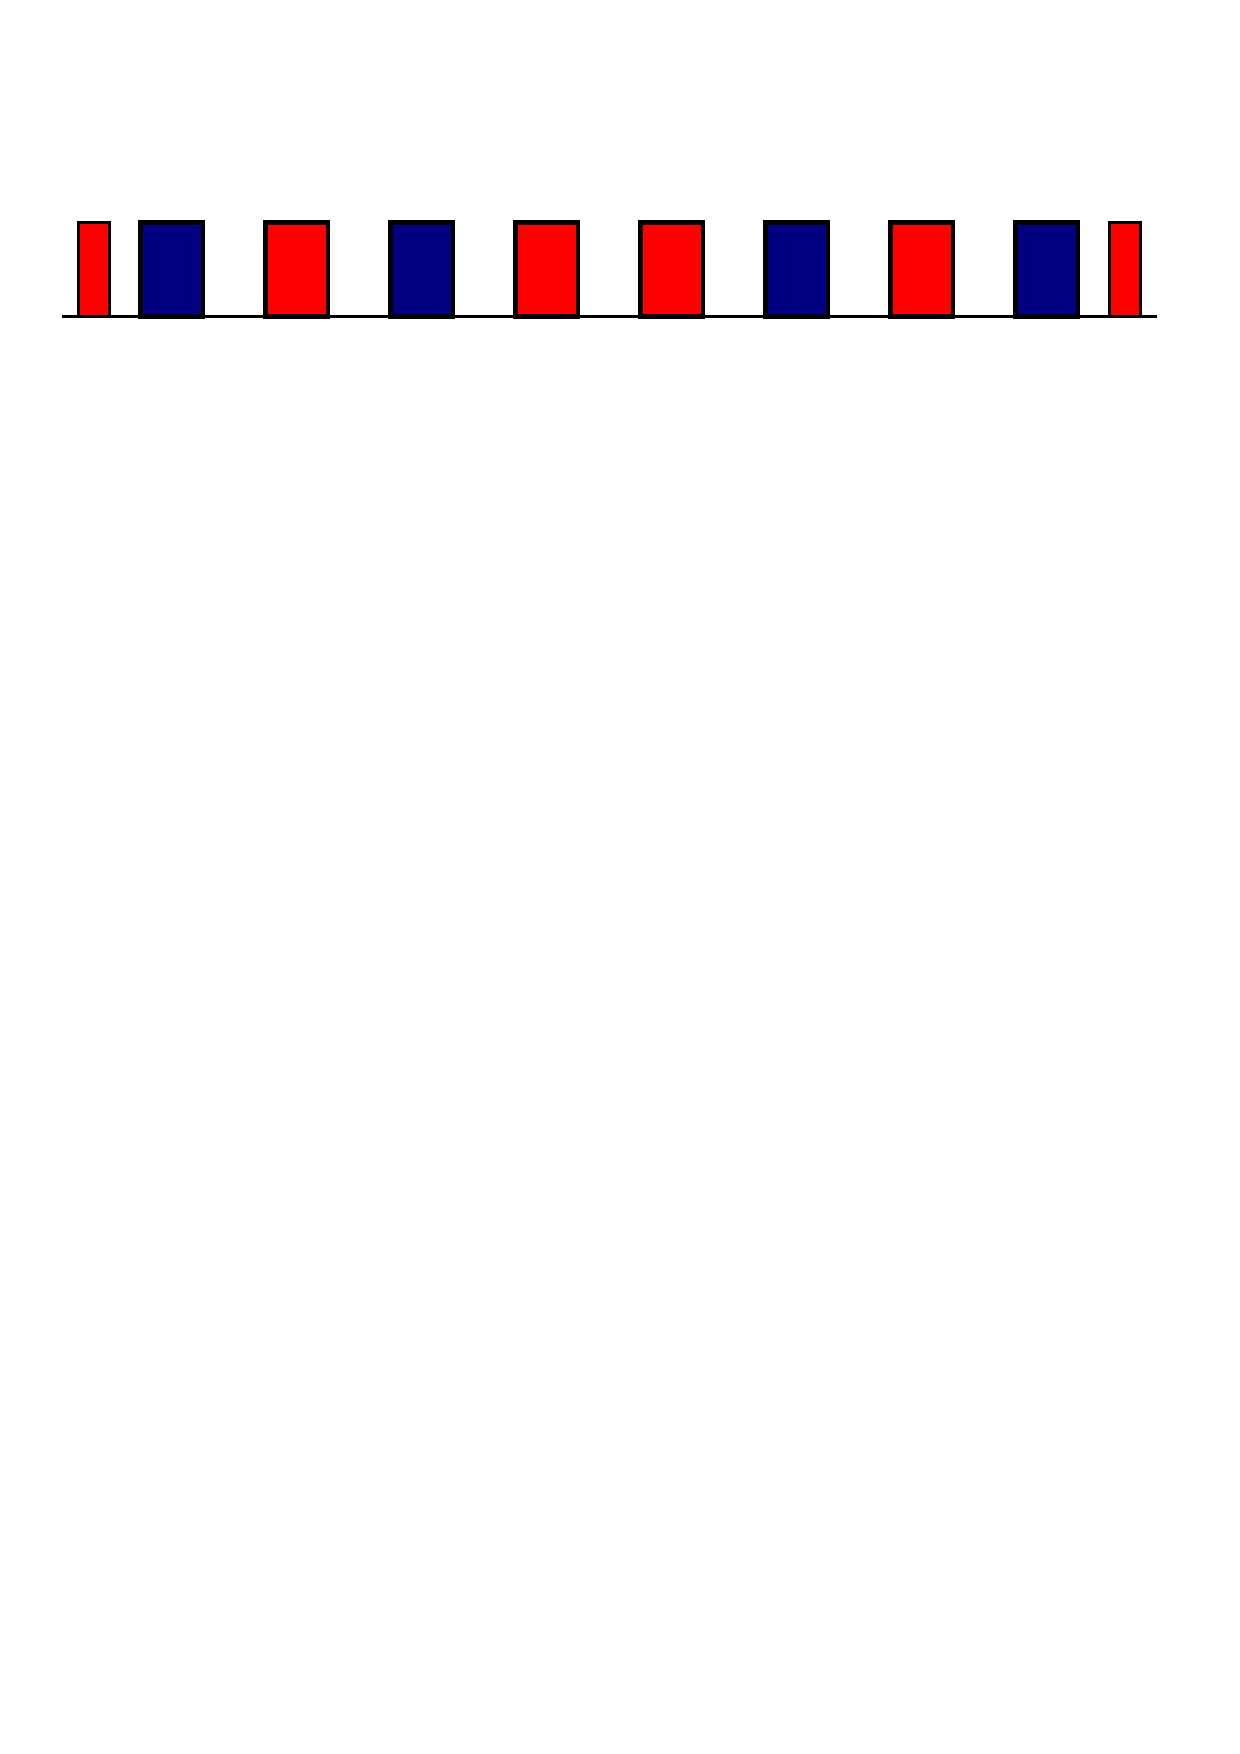
\includegraphics[scale=0.2]{XY82}
%	\end{figure}
%	
%	
%\end{columns}
%\end{frame}



\begin{frame}{Dynamical decoupling sequences}
\vspace{-1cm}
\begin{columns}[t]
	\column{.5\textwidth}
	\centering
	\begin{figure}
		\includegraphics[scale=0.2]{bulkhahn2.pdf}\vspace{-0.3cm}
		\caption{Hahn Echo: $T_2(t\leq 600\text{ns})$=(302$\pm$25)ns}
	\end{figure}
\begin{itemize}
	\item $T_2$ improvement up to factor 200 for CPMG
	\item $T_2$ increased by factor of about 90 for all XY
	\item CPMG outperforms XY
\end{itemize}
	
	\column{.5\textwidth}
	\centering
	\begin{figure}
		\includegraphics[scale=0.2]{xybulk2.pdf}\vspace{-0.3cm}
		\caption{XY on the bulk diamond}
	\end{figure}
\vspace{-1cm}
\begin{figure}
	\includegraphics[scale=0.2]{cpbulk2.pdf}
\vspace{-0.3cm}
	\caption{CPMG on the bulk diamond}
\end{figure}
\end{columns}
\end{frame}

\subsection{Spectral decomposition}

\begin{frame}{Spectral decomposition}

\begin{itemize}
	\item loss  of coherence can be described using
	\begin{equation}\nonumber
	C(t)=e^{-\chi(t)}
	\end{equation}
	with\footnotemark[1]
	
	
	\begin{equation}\nonumber
	\chi(t)=\frac{1}{\pi}\int^{\infty}_0d\omega S(\omega)\frac{F(\omega t)}{\omega^2}
	\end{equation}
	
	$F(\omega t)$ filter function,$S(\omega)$ spectral density function
	
	\item $S(\omega)$ assumed to have Lorentzian shape\footnotemark[1]:   \begin{equation}\nonumber
	S(\omega)=\frac{\Delta^2\tau_c}{\pi}\frac{1}{1+(\omega\tau_c)^2}
	\end{equation}  
	$\Delta$ average coupling strength  of spin bath to the probed NVs,\\ $\tau_c$ correlation time of N bath spins with each other
\end{itemize}
\footnotetext[1]{{N. Bar-Gill et al., "Suppression of spin-bath dynamics for improved coherence of multi-spin-qubit systems,"\textit{ Nature Communications 3, Article number: 858},
		2012.}}
\end{frame}

\begin{frame}{Spectral decomposition}
\vspace{-1cm}
\begin{columns}[t]
	\column{.5\textwidth}
	\centering
	\begin{figure}
		\includegraphics[scale=0.35]{ndc32.pdf}
		\caption{calculation for CPMG-32}
	\end{figure}
\vspace{-0.5cm}
	\begin{itemize}
		\item correlation between $\Delta$ and $\tau_c$
		\item for $\omega\ll\tau_c^{-1}$:
		\begin{equation}\nonumber
		S(\omega)=\frac{\Delta^2\tau_c}{\pi}
		\end{equation}
	\end{itemize}
	
	\column{.5\textwidth}
	\centering
	\begin{figure}
		\includegraphics[scale=0.35]{nd122.pdf}\caption{spectral densities for all sequences}
	\end{figure}
	\vspace{-1cm}
	\begin{table}[H]
		\centering
		\scalebox{0.9}{
			\begin{tabular}{l|ll|l}
				sequence & $\tau_c${[}ns{]} & $\Delta${[}MHz{]} 
			 \\\hline
				Hahn     & 66               & 18                \\
				CPMG-8   & 89               & 8                  \\
				CPMG-16  & 10               & 18                         \\
				CPMG-32  & 32               & 7                            \\
				CPMG-64  & 125              & 4                           
		\end{tabular}}
	\end{table}
\end{columns}

\end{frame}

\begin{frame}{Spectral decomposition}
\vspace{-1cm}
\begin{columns}[t]
	\column{.5\textwidth}
	\centering
	\begin{figure}
		\includegraphics[scale=0.35]{hahnbulk.pdf}\vspace{-0.3cm}
		\caption{calculation for Hahn}
	\end{figure}
\vspace{-0.5cm}
	\begin{itemize}
		\item same correlation as before
		\item similar experiments\footnotemark[1]
	: 1MHz$\leq\Delta\leq$10MHz and 
		1$\mu$s$\leq\tau_c\leq$15$\mu$s
	\end{itemize}
	
	\column{.5\textwidth}
	\centering
	\begin{figure}
		\includegraphics[scale=0.35]{bd124.pdf}\vspace{-0.3cm}
		\caption{spectral densities for all sequences}
	\end{figure}
	\vspace{-0.5cm}
	\begin{table}[H]
		\centering
		\scalebox{0.9}{
			\begin{tabular}{l|ll}
				sequence & $\tau_c${[}ns{]} & $\Delta${[}MHz{]} \\\hline
				Hahn     & 69               & 95                       \\
				CPMG-4   & 700               & 2.2                              \\
				CPMG-8  & 650               & 2.3                             \\
				CPMG-16  & 250               & 2.5                     \\
				CPMG-32  & 370              & 1.7                      
		\end{tabular}}
	\end{table}
\end{columns}
\vspace{-0.5cm}
\footnotetext[1]{{N. Bar-Gill et al., "Suppression of spin-bath dynamics for improved coherence of multi-spin-qubit systems," \textit{Nature Communications 3, Article number: 858}, 2012.}}
\end{frame}

\section{Conclusion and Outlook}
\begin{frame}{Conclusion and Outlook}
\begin{itemize}
\item successful implementation of DD protocols
\item CPMG outperforms XY
\item improvement of factor 50 in nanodiamond and 200 in bulk diamond $\rightarrow$ $T_2=50\mu$s
\item spectral density analysis provided information about the surrounding magnetic environment
\item sensitivity:
\begin{equation}\nonumber
\eta=\frac{\pi\hbar}{2 g\mu_B C\sqrt{N\cdot T_2}}
\end{equation}
$\rightarrow$  $\eta_{ND}\approx$ 10nT/$\sqrt{Hz}$, $\eta_{BD}\approx$(6-18)nT/$\sqrt{Hz}$
\item error sources: BPG (pulse errors), MW splitter, AOM
\item future:
\begin{itemize}
\item better time and phase control
\item implementation of other decoupling protocols
%\nocite{avc}\nocite{bel}\nocite{cfm}\nocite{cmmem}\nocite{cod}\nocite{czj}\nocite{darm}\nocite{dd}\nocite{ddsc}\nocite{dgcvd}\nocite{ess}\nocite{gmf}\nocite{hpht}\nocite{hted}\nocite{lar}\nocite{mspd}\nocite{nd}\nocite{nmr}\nocite{nvref}\nocite{opdadh}\nocite{pea}\nocite{pod}\nocite{poo}\nocite{qc}\nocite{qdd}\nocite{qm}\nocite{qmg}\nocite{qr}\nocite{qtl}\nocite{rdc}\nocite{sas}\nocite{sas2}\nocite{sdd}\nocite{st}\nocite{ttwo}\nocite{squid}
\end{itemize}
\end{itemize}
\end{frame}
\end{document}

